\documentclass{standalone}
\usepackage{tikz}
\usepackage{pgfplots}
\usepackage{amsmath}  % For \text{M} if needed

\pgfplotsset{compat=1.18}  % To avoid the warning about compatibility

\begin{document}
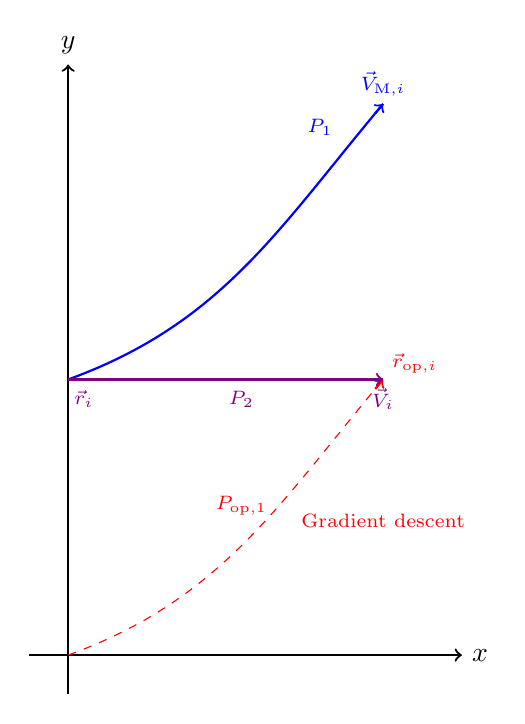
\begin{tikzpicture}[xshift=0.25cm, scale=1]

    % Axes with slightly extended lines to match the cross at origin in xbin
    \draw[thick,->] (-0.5,-3.5) -- (5,-3.5) node[right] {$x$}; % Extended x-axis left of origin
    \draw[thick,->] (0,-4) -- (0,4) node[above] {$y$}; % Aligned "y" label directly on top of the arrow
    
    % Inward concave curve
    \draw[thick,blue] (0,0) to [out=20,in=230] (4,3.5);
    \draw[dashed,red] (0,-3.5) to [out=20,in=230] (4,0);
    \draw[thick,violet] (0,0) to (4,0);
    
    % Arrow at the end of the curve
    \draw[thick,->,blue] (3.9,3.38) -- (4,3.5);
    \draw[thick,->,red] (3.9,-0.12) -- (4,0);
    \draw[thick,->,violet] (0,0) -- (4,0);
    
    %\draw[dashed,->, red] (4,3.5) -- (4,0); 
    
    % Labels
    \node[font=\scriptsize, color=blue] at (3.2, 3.2) {$P_1$};
    \node[font=\scriptsize, color=violet] at (2.2, -0.25) {$P_2$};
    \node[font=\scriptsize, color=red] at (2.2, -1.6) {$P_{\text{op},1}$};
    \node[font=\scriptsize, color=red] at (4, -1.8) {Gradient descent};
    \node[font=\scriptsize, color=violet] at (0.2, -0.25) {$\vec{r}_i$};
    \node[font=\scriptsize, color=blue] at (4, 3.75) {$\vec{V}_{\text{M},i}$};
    \node[font=\scriptsize, color=violet] at (4, -0.25) {$\vec{V}_{i}$}; 
    \node[font=\scriptsize, color=red] at (4.4, 0.2) {$\vec{r}_{\text{op},i}$}; 
\end{tikzpicture}
\end{document}
